\documentclass{article}
%Usepackages
\usepackage{adjustbox, amsmath, amssymb, amsthm, blindtext, bm, bbm, dblfloatfix, esint, fancyhdr, float, graphicx, letltxmacro, marginnote, mathtools, subcaption, xcolor, titlesec, esint}
\usepackage{amssymb}
\usepackage[font={small, it}]{caption}
\usepackage{amsmath}
\usepackage{floatrow}
\usepackage{times}
\usepackage{ stmaryrd }
\usepackage{amsthm}
\usepackage{xcolor}
\usepackage{mathrsfs}
\usepackage[colorlinks = true,
            linkcolor = black,
            urlcolor  = blue,
            citecolor = black,
            anchorcolor = blue]{hyperref}
% \usepackage[mathscr]{euscript}
\usepackage{mathrsfs}
\usepackage{wasysym}
%\usepackage{pxfonts}
\usepackage[letterpaper, portrait, margin=1in]{geometry}
\usepackage{graphicx}
\usepackage{tikz}
\usepackage{tikz-3dplot}
\usepackage{pgfplots}
\usetikzlibrary{decorations.pathmorphing,patterns}
\usepackage{lipsum}
\usepackage{float}
\usepackage{subcaption}
\usepackage[object=vectorian]{pgfornament}
\usepackage{mwe}
\usepackage{bigints}
\usepackage{csquotes}
\usepackage{titlesec}
\usepackage{halloweenmath}
\setcounter{secnumdepth}{4}
\titleformat{\paragraph}
{\normalfont\normalsize\bfseries}{\theparagraph}{1em}{}
\titlespacing*{\paragraph}
{0pt}{3.25ex plus 1ex minus .2ex}{1.5ex plus .2ex}
\usepackage{mathtools}
\usepackage{pgfplots}
\pgfplotsset{compat=1.15}
\usepackage{lastpage}
\usepackage{enumitem}
\usepackage{tensor}
\usepackage{mathtools}

% This is for the header:
% https://tex.stackexchange.com/questions/75168/get-current-section-name-without-label
\usepackage{nameref}
\makeatletter
\newcommand*{\currentname}{\@currentlabelname}
\makeatother

\usepackage{fancyhdr} 
    \pagestyle{fancy}
    \fancyhf{}
    \fancyhead[R]{ Page \thepage \  of \pageref{LastPage}}
    \fancyhead[L]{\currentname}
\usepackage{setspace}
\usepackage{tikz}
\usetikzlibrary{hobby}

\usepackage{pst-node}
\usepackage{tikz-cd}
\usepackage[most]{tcolorbox}

% \makeatletter
% \renewcommand\@endtheorem{\vvv@endmarker\endtrivlist\@endpefalse}
% \newcommand\vvv@endmarker{%
%   {\unskip\nobreak\hfil\penalty50
%   \hskip2em\vadjust{}\nobreak\hfil\openbox
%   \parfillskip=0pt \finalhyphendemerits=0 \par
%   \penalty 10000 \parskip=0pt\noindent}\ignorespaces}
% \makeatother

\theoremstyle{definition}

% https://tex.stackexchange.com/questions/616586/how-to-make-a-tcolorbox-with-only-a-left-side-rule


\newtheorem{thm}{Theorem}[section]
\newtheorem{defn}[thm]{Definition}
\newtheorem{exmp}[thm]{Example}
\newtheorem{lem}[thm]{Lemma}
\newtheorem{conjecture}[thm]{Conjecture}
\newtheorem{exercise}[thm]{Exercise}
\newtheorem{fact}[thm]{Fact}
\newtheorem{claim}[thm]{Claim}
\newtheorem{cor}[thm]{Corollary}
\newtheorem{summary}[thm]{Summary}

\newtheorem{idea}[thm]{Idea}
\newtheorem{application}[thm]{Application}
\newtheorem{rmk}[thm]{Remark}

\newtheorem{prop}[thm]{Proposition}
\newtheorem{ques}[thm]{Question}

\newtcolorbox{cbox}[1][]{
            breakable,
            boxrule=0pt,
            frame hidden,
            sharp corners,
            enhanced,
            borderline west={2pt}{0pt}{#1},
            colback=#1!5!white}

% \newenvironment{cthm}[3]
%     {\begin{cbox}[#2]
%     \color{#2}
%     \begin{#3}[#1]
%     \color{black}
%     }
%     {
%     \end{#3} 
%     \end{cbox}
%     }

% \newenvironment{theorem}[1][]
% {\begin{cthm}{#1}{orange}{thm}}
% {\end{cthm}}

\newenvironment{theorem}[1][]
    {\begin{cbox}[blue]
    \color{blue}
    \begin{thm}[#1]
    \color{black}
    }
    {
    \end{thm} 
    \end{cbox}
    }

\newenvironment{corollary}[1][]
    {\begin{cbox}[orange]
    \color{orange}
    \begin{cor}[#1]
    \color{black}
    }
    {
    \end{cor} 
    \end{cbox}
    }

\newenvironment{lemma}[1][]
    {\begin{cbox}[orange]
    \color{orange}
    \begin{lem}[#1]
    \color{black}
    }
    {
    \end{lem} 
    \end{cbox}
    }

\newenvironment{proposition}[1][]
    {\begin{cbox}[orange]
    \color{orange}
    \begin{prop}[#1]
    \color{black}
    }
    {
    \end{prop} 
    \end{cbox}
    }

\newenvironment{definition}[1][]
    {\begin{cbox}[red]
    \color{red}
    \begin{defn}[#1]
    \color{black}
    }
    {
    \end{defn} 
    \end{cbox}
    }

\newenvironment{example}[1][]
    {\begin{cbox}[violet]
    \color{violet}
    \begin{exmp}[#1] \color{black}
    }
    {
    \end{exmp} 
    \end{cbox}
    }

\newenvironment{question}[1][]
    {\begin{cbox}[black]
    \begin{ques}[#1]
    }
    {
    \end{ques} 
    \end{cbox}
    }

\newenvironment{remark}[1][]
    {\begin{cbox}[black]
    \begin{rmk}[#1]
    }
    {
    \end{rmk} 
    \end{cbox}
    }



\newenvironment{solution}
  {\renewcommand\qedsymbol{$\blacksquare$}\begin{proof}[Solution]}
  {\end{proof}}
\newenvironment{answer}
  {\begin{proof}[Answer]}
  {\end{proof}}
  
% \newenvironment{example}
%   {\pushQED{\qed}\renewcommand{\qedsymbol}{$\triangle$}\examplex}
%   {\popQED\endexamplex}


%%%%%%%%%%%%%%%%%%%%%%%%%%%%%

%Custom Commands
    \renewcommand\qedsymbol{$\blacksquare$}
    \newcommand{\Pcal}{\mathcal{P}}
    \newcommand{\ve}{\varepsilon}
    \newcommand{\Ocal}{\mathcal{O}}
    \newcommand{\Asf}{\textsf{A}}
    \newcommand{\al}{\alpha}
    \newcommand{\be}{\beta}
    \newcommand{\Nbb}{\mathbb{N}}
    \newcommand{\Si}{\Sigma}
    \newcommand{\Hbb}{\mathbb{H}}
    \DeclareMathOperator{\diag}{diag}
    \newcommand{\De}{\Delta}
    \newcommand{\Xcal}{\mathcal{X}}
    \newcommand{\si}{\sigma}
    \newcommand{\Ga}{\Gamma}
    \newcommand{\Cscr}{\mathscr{C}}
    \newcommand{\1}{\mathbf{1}}
    \newcommand{\Dcal}{\mathcal{D}}
    \newcommand{\Iscr}{\mathscr{I}}
    \newcommand{\Pbb}{\mathbb{P}}
    \newcommand{\B}{\mathbb{B}}
    \newcommand{\Dscr}{\mathscr{D}}
    \newcommand{\Nfrak}{\mathfrak{N}}
    \newcommand{\Efrak}{\mathfrak{E}}
    \DeclareMathOperator{\charp}{charpoly}
    \newcommand{\Csf}{\mathsf{C}}
    \newcommand{\rfrak}{\mathfrak{r}}
    \newcommand{\Sbb}{\mathbb{S}}
    \newcommand{\La}{\Lambda}
    \newcommand{\de}{\delta}
    \DeclareMathOperator{\inte}{int}
    \DeclareMathOperator{\ord}{ord}
    \newcommand{\set}{\mathsf{set}}
    \newcommand{\Bscr}{\mathscr{B}}
    \newcommand{\Zscr}{\mathscr{Z}}
    \newcommand{\ab}{\mathrm{ab}}
    \newcommand{\Xscr}{\mathscr{X}}
    \newcommand{\Escr}{\mathscr{E}}
    \newcommand{\Gscr}{\mathscr{G}}
    \DeclareMathOperator{\Sym}{Sym}
    \newcommand{\om}{\omega}
    \newcommand{\gfrak}{\mathfrak{g}}
    \newcommand{\hfrak}{\mathfrak{h}}
    \newcommand{\kfrak}{\mathfrak{k}}
    \newcommand{\Grp}{\mathsf{Grp}}
    \newcommand{\Ab}{\mathsf{Ab}}
    \newcommand{\xbar}{\bar{x}}
    \newcommand{\abar}{\bar{a}}
    \newcommand{\ybar}{\bar{y}}
    \DeclareMathOperator{\coker}{coker}
    \newcommand{\Modsf}{\mathsf{Mod}}
    \newcommand{\op}{\mathrm{op}}
    \newcommand{\Ring}{\mathsf{Ring}}
    \newcommand{\modsf}{\mathsf{mod}}
    \DeclareMathOperator{\Alt}{Alt}
    \newcommand{\Om}{\Omega}
    \newcommand{\ze}{\zeta}
    \newcommand{\Fcal}{\mathcal{F}}
    \newcommand{\Oscr}{\mathscr{O}}
    \newcommand{\gl}{\mathfrak{gl}}
    \DeclareMathOperator{\Lie}{Lie}
    \DeclareMathOperator{\GL}{GL}
    \DeclareMathOperator{\SL}{SL}
    \DeclareMathOperator{\Vol}{Vol}
    \DeclareMathOperator{\Disc}{Disc}
    \DeclareMathOperator{\SO}{SO}
    \newcommand{\Xfrak}{\mathfrak{X}}
    \DeclareMathOperator{\id}{id}
    \DeclareMathOperator{\Int}{Int}
    \DeclareMathOperator{\End}{End}
    \DeclareMathOperator{\Aut}{Aut}
    \DeclareMathOperator{\stab}{stab}
    \DeclareMathOperator{\orb}{orb}
    \DeclareMathOperator{\grad}{grad}
    \DeclareMathOperator{\curl}{curl}
    \newcommand{\vp}{\varphi}
    \newcommand{\vt}{\vartheta}
    \DeclareMathOperator{\Gal}{Gal}
    \DeclareMathOperator{\rank}{rank}
    \DeclareMathOperator{\col}{col}
    \DeclareMathOperator{\Tame}{Tame}  
    \newcommand{\Yscr}{\mathscr{Y}}
    \newcommand{\Fbb}{\mathbb{F}}
    \newcommand{\Hcal}{\mathcal{H}}
    \newcommand{\arctanh}{\text{arctanh}}
    \newcommand{\pa}{\partial}
    \newcommand{\del}{\boldsymbol{\nabla}}
    \newcommand{\na}{\nabla}
    \newcommand{\Ycal}{\mathcal{Y}}
    \DeclareMathOperator{\spn}{span}
    \DeclareMathOperator{\Inn}{Inn}
    \DeclareMathOperator{\chara}{char}
    \newcommand{\lap}{\nabla^2}
    \newcommand{\Pfrak}{\mathfrak{P}}
    \newcommand{\mfrak}{\mathfrak{m}}
    \newcommand{\Fvec}{\mathbf{F}}
    \newcommand{\Mcal}{\mathcal{M}}
    \newcommand{\ellvec}{\boldsymbol{\ell}}
    \newcommand{\rvec}{\mathbf{r}}
    \DeclareMathOperator{\supp}{supp}
    \newcommand{\Abb}{\mathbb{A}}
    \newcommand{\svec}{\mathbf{s}}
    \newcommand{\VECT}{\mathsf{VECT}}
    \newcommand{\fs}{\vec{\sigma}}
    \newcommand{\bs}{\cev{\sigma}}
    \newcommand{\uvec}{\mathbf{u}}
    \newcommand{\iunit}{\boldsymbol{\hat{\i}}}
    \newcommand{\junit}{\boldsymbol{\hat{\j}}}
    \newcommand{\xunit}{\mathbf{\hat{x}}}
    \newcommand{\Char}{\text{char}}
    \newcommand{\kunit}{\mathbf{\hat{k}}}
    \newcommand{\theunit}{\boldsymbol{\hat{\theta}}}
    \newcommand{\pvec}{\mathbf{p}}
    \newcommand{\qvec}{\mathbf{q}}
    \newcommand{\Qcal}{\mathcal{Q}}
    \newcommand{\yvec}{\mathbf{y}}
    \newcommand{\xvec}{\mathbf{x}}
    \newcommand{\wvec}{\mathbf{w}}
    \newcommand{\bvec}{\mathbf{b}}
    \newcommand{\Ucal}{\mathcal{U}}
    \newcommand{\Ncal}{\mathcal{N}}
    \newcommand{\Scal}{\mathcal{S}}
    \newcommand{\Nscr}{\mathscr{N}}
    \newcommand{\da}{\dagger}
    \newcommand{\CT}{\mathrm{H}}
    \newcommand{\Sscr}{\mathscr{S}}
    \DeclareMathOperator{\lcm}{lcm}
    \newcommand{\evec}{\mathbf{e}}
    \newcommand{\Kscr}{\mathscr{K}}
    \newcommand{\ebold}{\boldsymbol{e}}
    \newcommand{\zvec}{\mathbf{z}}
    \newcommand{\vvec}{\mathbf{v}}
    \newcommand{\Tscr}{\mathscr{T}}
    \newcommand{\avec}{\mathbf{a}}
    \newcommand{\Avec}{\mathbf{A}}
    \newcommand{\Ivec}{\mathbf{I}}
    \newcommand{\ivec}{\mathbf{i}}
    \newcommand{\jvec}{\mathbf{j}}
    \newcommand{\kvec}{\mathbf{k}}
    \newcommand{\of}{\mathfrak{o}}
    \DeclareMathOperator{\Ot}{O}
    \DeclareMathOperator{\Sy}{S}
    \newcommand{\slf}{\mathfrak{sl}}
    \newcommand{\muvec}{\boldsymbol{\mu}}
    \newcommand{\Bvec}{\mathbf{B}}
    \newcommand{\Cvec}{\mathbf{C}}
    \newcommand{\eunit}{\mathbf{\hat{e}}}
    \newcommand{\vpunit}{\boldsymbol{\hat{\varphi}}}
    \newcommand{\zero}{\boldsymbol{0}}
    \newcommand{\tauvec}{\boldsymbol{\tau}}
    \newcommand{\runit}{\mathbf{\hat{r}}}
    \newcommand{\U}{\mathcal{U}}
    \newcommand{\Zbb}{\mathbb{Z}}
    \newcommand{\Bsf}{\mathsf{B}}
    \DeclareMathOperator{\G}{G}
    \newcommand{\gmat}{\textsf{g}}
    \newcommand{\Ccal}{\mathcal{C}}
    \newcommand{\SM}{\mathsf{SM}}
    \newcommand{\VB}{\mathsf{VB}}
    \newcommand{\Dsf}{\mathsf{D}}
    \newcommand{\Fscr}{\mathscr{F}}
    \DeclareMathOperator{\Map}{Map}
    \DeclareMathOperator{\Frob}{Frob}
    \newcommand{\Imat}{\textsf{I}}
    \newcommand{\Rmat}{\textsf{R}}
    \DeclareMathOperator{\Frac}{Frac}
    \DeclareMathOperator{\Spec}{Spec}
    \DeclareMathOperator{\Emb}{Emb}
    \newcommand{\Kcal}{\mathcal{K}}
    \newcommand{\Wcal}{\mathcal{W}}
    \newcommand{\Lcal}{\mathcal{L}}
    \newcommand{\Tcal}{\mathcal{T}}
    \newcommand{\Ecal}{\mathcal{E}}
    \DeclareMathOperator{\im}{im}
    \newcommand{\Qbb}{\mathbb{Q}}
    \newcommand{\ga}{\gamma}
    \newcommand{\la}{\lambda}
    \newcommand{\RomanNumeralCaps}[1]
        {\MakeUppercase{\romannumeral #1}} 
    \newcommand{\dif}{\text{d}}
    \newcommand{\Rbb}{\mathbb{R}}
    \newcommand{\Tbb}{\mathbb{T}}
    \DeclareMathOperator{\Hom}{Hom}
    \DeclareMathOperator{\conv}{conv}
    \newcommand{\Vcat}{\mathsf{V}}
    \newcommand{\Gr}{\text{Gr}}
    \newcommand{\Bcal}{\mathcal{B}}
    \newcommand{\Acal}{\mathcal{A}}
    \newcommand{\pfrak}{\mathfrak{p}}
    \newcommand{\qfrak}{\mathfrak{q}}
    \newcommand{\Evec}{\mathbf{E}}
    \newcommand{\omvec}{\boldsymbol{\omega}}
    \newcommand{\alvec}{\boldsymbol{\alpha}}
    \newcommand{\gvec}{\mathbf{g}}
    \newcommand{\afrak}{\mathfrak{a}}
    \newcommand{\bfrak}{\mathfrak{b}}
    \newcommand{\Cbb}{\mathbb{C}}
    \newcommand{\gavec}{\boldsymbol{\gamma}}
    \newcommand{\Tvec}{\mathbf{T}}
    \newcommand{\Vscr}{\mathscr{V}}
    \newcommand{\Ascr}{\mathscr{A}}
    \newcommand{\Uscr}{\mathscr{U}}
    \newcommand{\Sfrak}{\mathfrak{S}}
    \DeclareMathOperator{\sgn}{sgn}
    \DeclareMathOperator{\vol}{vol}
    \newcommand{\Pscr}{\mathscr{P}}
    \newcommand{\Wscr}{\mathscr{W}}
    \newcommand{\bcdot}{\boldsymbol{\cdot}}
    \DeclareMathOperator{\tr}{tr}
    
    \newcommand{\sectionline}{
        \noindent
        \begin{center}
        {
        {{
        {\begin{tikzpicture}
        \node  (C) at (0,0) {};
        \node (D) at (16,0) {};
        \path (C) to [ornament=89] (D);
        \end{tikzpicture}}}}}
        \end{center}
        }
    \newcommand{\sectionlineflip}{
        \noindent
        \begin{center}
        {
        {{
        {\begin{tikzpicture}
        \node  (C) at (0,0) {};
        \node (D) at (16,0) {};
        \path (D) to [ornament=89] (C);
        \end{tikzpicture}}}}} 
        \end{center}
        }
        

        
       
%%%%%%%%%%%%%%%%%%%%%%%%%%%%%%%
%Custom Symbols
\newcommand{\goodemptyset}[1]{%
\begin{tikzpicture}[#1]%
\draw (0,0) circle (0.1);%
\draw(-0.07,-0.14)--(0.07,0.14);
\end{tikzpicture}%
}

\newcommand{\es}{\raisebox{-1pt}{\goodemptyset{}}}


\makeatletter
\DeclareRobustCommand{\cev}[1]{%
  {\mathpalette\do@cev{#1}}%
}
\newcommand{\do@cev}[2]{%
  \vbox{\offinterlineskip
    \sbox\z@{$\m@th#1 x$}%
    \ialign{##\cr
      \hidewidth\reflectbox{$\m@th#1\vec{}\mkern4mu$}\hidewidth\cr
      \noalign{\kern-\ht\z@}
      $\m@th#1#2$\cr
    }%
  }%
}
\makeatother


\makeatletter
\DeclarePairedDelimiterX{\pmodx}[1]{(}{)}{{\operator@font mod}\mkern6mu#1}
\renewcommand{\pmod}{%
  \allowbreak
  \if@display\mkern18mu\else\mkern8mu\fi
  \pmodx
}
\makeatother
\DeclarePairedDelimiter\bra{\langle}{\rvert}
\DeclarePairedDelimiter\ket{\lvert}{\rangle}
\DeclarePairedDelimiterX\braket[2]{\langle}{\rangle}{#1 \delimsize\vert #2}

 
\makeatletter
\newcommand{\colim@}[2]{%
  \vtop{\m@th\ialign{##\cr
    \hfil$#1\operator@font colim$\hfil\cr
    \noalign{\nointerlineskip\kern1.5\ex@}#2\cr
    \noalign{\nointerlineskip\kern-\ex@}\cr}}%
}
\newcommand{\colim}{%
  \mathop{\mathpalette\colim@{\rightarrowfill@\scriptscriptstyle}}\nmlimits@
}
\renewcommand{\varinjlim}{%
  \mathop{\mathpalette\varlim@{\rightarrowfill@\scriptscriptstyle}}\nmlimits@
}
\renewcommand{\varprojlim}{%
  \mathop{\mathpalette\varlim@{\leftarrowfill@\scriptscriptstyle}}\nmlimits@
}

\newcommand{\mjedit}[1]{{\color{orange}  #1}}
\newcommand{\mattie}[1]{{\color{orange} \sf $\clubsuit\clubsuit\clubsuit$ Mattie: [#1]}}
\newcommand{\margMa}[1]{\normalsize{{\color{red}\footnote{{\color{orange}#1}}}{\marginpar[{\color{red}\hfill\tiny\thefootnote$\rightarrow$}]{{\color{red}$\leftarrow$\tiny\thefootnote}}}}}
\newcommand{\Mattie}[1]{\margMa{(Mattie) #1}}


% %%%%%%%%%%%%%%%%%%%%%%%%%%%%%
% %Just arrows (cause normy arrows suck)
% \newcommand{\goodarrow}[1]{
% \begin{tikzpicture}[#1]
% \draw[-stealth] (0,0)--(0.4,0);
% \end{tikzpicture}
% }

% \renewcommand{\to}{\raisebox{2.4pt}{\hspace{0.08cm}\goodarrow{}\hspace{0.06cm}}}

% %%%%

% \newcommand{\goodtwoheadrightarrow}[1]{
% \begin{tikzpicture}[#1]
% \draw[->>, >=stealth] (0,0)--(0.4,0);
% \end{tikzpicture}
% }

% \renewcommand{\twoheadrightarrow}{\raisebox{2.4pt}{\hspace{0.08cm}\goodtwoheadrightarrow{}\hspace{0.06cm}}}

% %%%

% \newcommand{\goodhookrightarrow}[1]{
% \begin{tikzpicture}[#1]
% \draw[right hook-stealth] (0,0)--(0.4,0);
% \end{tikzpicture}
% }

% \renewcommand{\hookrightarrow}{\raisebox{2.3pt}{\hspace{0.08cm}\goodhookrightarrow{}\hspace{0.06cm}}}

% %%%

% \newcommand{\goodmapsto}[1]{
% \begin{tikzpicture}[#1]
% \draw[-stealth] (0,0)--(0.4,0);
% \draw[] (0,0.06)--(0,-0.06);
% \end{tikzpicture}
% }

% \renewcommand{\mapsto}{\raisebox{0pt}{\hspace{0.02cm}\goodmapsto{}\hspace{0.03cm}}}


% %%%%%%%%%%%%%%%%%%%%%%%%%%%%%

% \tikzcdset{arrow style=tikz, diagrams={>={stealth[round,length=4pt,width=4.5pt,inset=2.75pt]}}}






\renewcommand*\contentsname{Table of Content}

\title{APMA 2550: Numerical Solutions (Approximation) of PDEs I}
\author{Notes taken by Mattie Ji}
\date{Updated \today}
\setlength\parindent{0pt}

\begin{document}

\maketitle
These are lecture notes from \textbf{APMA 2550: Numerical Solutions (Approximation) of PDEs I} with Professor Mark Ainsworth at Brown University for the Fall 2023 semester. The most up-to-date version of the notes are maintained under my GitHub \href{https://github.com/maroon-scorch}{repository}.\\

These notes are taken by Mattie Ji with gracious help and input from the instructor of this course. If you find any mistakes in these notes, please feel free to direct them via email to me or send a pull request on GitHub.\\

The notes are last updated \today.
\tableofcontents
\newpage

\section{Lecture 1}

\subsection{Logistics}

\begin{itemize}
    \item \textbf{When: } We meet at Barus and Holley $3:00 - 5:20$ pm every Wednesday. We will take a $10$ minute break in the middle of lecture.
    \item \textbf{Assessment: } The grade of the class is divided into 2 components: Coursework is $80\%$ and the Final Project is $20\%$.
    
    Courseworks are homeworks assigned each Wednesday and due the following Wednesday before class. They are not meant to be busy work but as complementary materials for the course that might be challenging. Professor Ainsworth strongly believes in learning by doing assignments.

    We have a final project in this course because this class is to train future researchers. The final project itself will be more of computational nature and may have some applications.
    
    \item \textbf{Syllabus and Books: }

    \begin{remark}
    This is Professor Ainsworth's first time teaching this course. He has taught Part II and III before, but this is his first time teaching Part I. This is because, apparently, this class gets a lot of feedback as being ``boring". Another source of frustation is whenever he has a time-dependnet PDE, he would like his students to know how to solve it, but apparently past iterations of Part I never taught this. 
    \end{remark}

    The focus of this course is on time-discretization methods, ie. we want to solve time dependent PDEs/ODEs. This is a very classical topic and is so successful that barely anyone does research in this field anymore, but there are some very nice methods for us to know in this class.

    There are no recommended textbooks for this course, but there are some books you may consider:
    \begin{enumerate}
        \item J. D. Lambert, \textit{Numerical Methods for Ordinary Differential Systems: The Initial Value Problem}
        \item Volumes I to III of $\{$Hairer, Noursett, Wanner, Lubich$\}$, all about 500 pages each.
        \item Lots of other books...
    \end{enumerate}

    \item \textbf{Programming Languages for this class: }
    \begin{enumerate}
        \item What the instructor personally prefers: \texttt{C++}
        \item What the students can use: \texttt{Julia}, \texttt{Python}, \texttt{Matlab} (it would be alright for the class but instructor does not recommend), \texttt{C++}, \texttt{Fortran}, \texttt{ADA}.
        \item \texttt{Maple} and \texttt{Mathematica} aren't really recommended since they are algebraic manipulation packages and is not good at memory handling.
    \end{enumerate}

    \item \textbf{Prerequisites: } 
    \begin{enumerate}
        \item Working knowledge of real analysis. We will have theoretical portions in this class.
     \begin{remark}
        The \textbf{Sleipner C Oil Platform} was an incident where an oil field blew up (it measured a $5$ on the earthquake Richter scale. What happened was the numerical analysts used a completely incorrect method to do the calculations. A lot of workers involved were sent to jail due to professional negligence. This is why we care about the ``analysis" part of numerical analysis.
    \end{remark}
        \item Some familiarity with programming.
        \item You have seen ODEs and PDEs before.
    \end{enumerate}
    But we will cover some relevant contents in these topics when needed.
\end{itemize}


\subsection{Ordinary Differential Equations}

ODEs arise naturally whenever we model any time dependent system.

\begin{example}[Cooling of a Body]
Suppose we have a cup of tea with temperature $u(t)$ at time $t$. The ambient temperature is $T$ that we assume is lower than $u(t)$. In this case, tea cools because the ambient temperature is lower than $u(t)$.
\[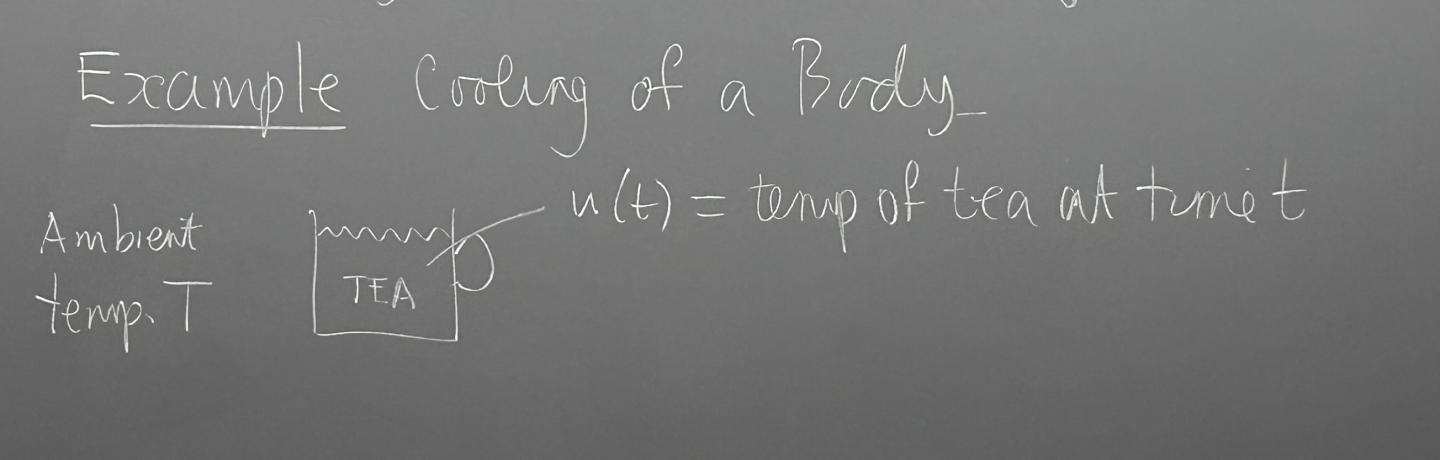
\includegraphics[width=0.6\textwidth]{Figures/lecture1/lec1-1.png}\]
Consider the system at time $t$ and time $t + \delta t$. Hear energy is conserved in this system. The heat energy in the cup at time $t$
 is
 \[m_T c_T u(t)\]
 where $m_T$ is the mass of the tea and $c_T$ is the specific heat capacity of the tea. The heat energy at time $t + \delta t$ is
 \[m_T c_T u(t + \delta t) = m_T c_T u(t) - \{\text{Heat lost to the surroundings}\}\]

\begin{question}
    How much heat is lost?
\end{question}

The amount of heat is lost should be dependent on the difference $u(t) - T$, the surface area of the cup, and should be proporitional to $\delta t$ (provided that it is really small so we can do a local linear approximation). There could also be vapor going out with some convection going out, but we will ignore it for now by Ainsworth's Principle of Maximum Laziness.\\

Hence the amount of heat lost could be modeled as
\[\alpha (u(t) - T) \delta t\]
where $\alpha > 0$ is some constant that measures the ``physical attributes" of the cup.\\

Hence, the heat energy at time $t + \delta t$ can be given as
\[m_T c_T u(t + \delta t) = m_T c_T u(t) - \alpha (u(t) - T) \delta t\]
This equation implies that
\[\frac{ u(t + \delta t) - u(t)}{\delta t} = - \beta (u(t) + T)\]
where $\beta = \frac{\alpha}{m_T c_T} > 0$. Taking the limit as $\delta t \to 0$, we have that
\[u'(t) = - \beta (u(t) - T)\]
Finally, we add an initial condition specifying that $u(t_0) = u_0$.\\

Solving the ODE using standard techniques of calculus, we obtained that
\[u(t) = T + (u_0 - T) e^{-\beta t}, t \geq 0\]

Observe that as $t \to \infty$, we have that
\[u(t) \to T\]

This question is an example of a linear, first order, initial value problem. This is called \textbf{Newton's Law of Cooling}.
 \end{example}

 \begin{example}
     What if we replace the cup of tea with the planetary phenonmenon ``black body"?
     \[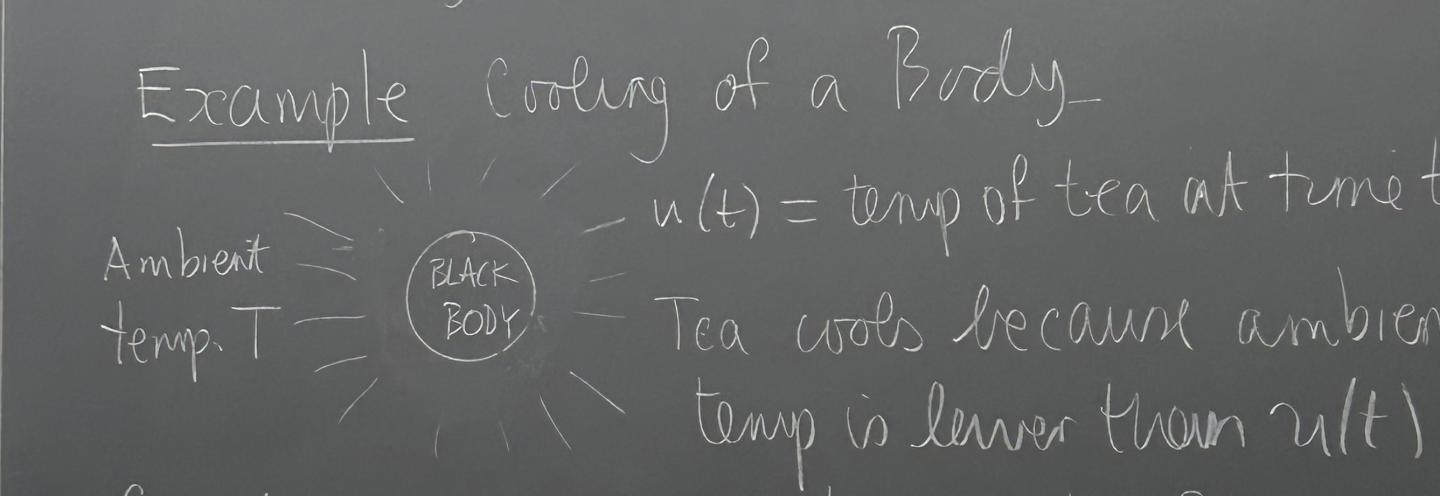
\includegraphics[width=0.6\textwidth]{Figures/lecture1/lec1-2.png}\]
     \textbf{Stefan's Law of Black Body Radiation} says that the heat energy lost should be proportional to $(u(t) - T)^4$ instead of $(u(t) - T)$ and we have
     \[\alpha_1 (u(t) - T) + \alpha_4 (u(t) - T)^4\]
     for $\alpha_1, \alpha_4 \geq 0$.\\

     This leads to an initial valued problem:
     \[u'(t) = - \beta_1 (u(t) - T) - \beta_4 (u(t) - T)^4, u(t_0) = u_0\]
     The solution of this can be done in analytic form, but it is not as easy as the previous example.
     \begin{question}
         How do we proceed from here? It depends on who you ask.
     \end{question}
     \begin{itemize}
         \item \textbf{Dynamical system approach: }In this case, we look for an equilibrium and cosnider the RHS
         \[f(u) = - \beta_1 (u - T) - \beta_4 (u - T)^4\]
         An equilibrium (critical point) is here if and only if $f(u) = 0$.
         
         For example $u = T$ is an example of a equilibrium. $\beta_1 + \beta_4 (u - T)^3 = 0$ is another solutions, which is true if and only if $u = T - (\frac{\beta_1}{\beta_4})^{1/3} < T$. These are the only two equilibriums of the system. The graph looks somewhat like:
       \[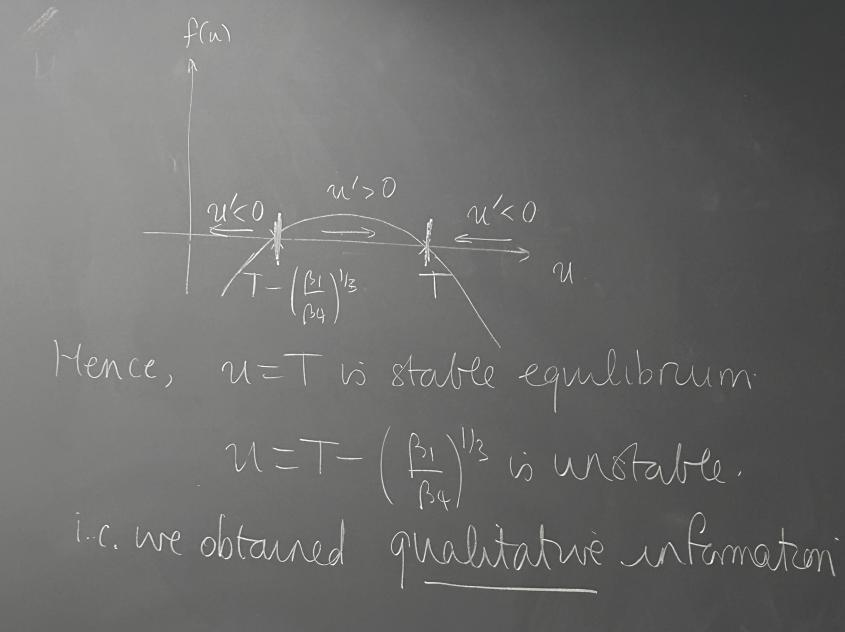
\includegraphics[width=0.6\textwidth]{Figures/lecture1/lec1-3.png}\]
        Hence, $u = T$ is a stable equilibrium and $u = T - (\frac{\beta_1}{\beta_4})^{1/3}$ is an unstable equilibrium. We have obtained \textbf{qualitative information} about the system. However, sometimes we need \textbf{quantitative information} about a system, ie. we want a sufficiently accurate approximatin of this solution.
        
        The physics is also a little dodgy for $t < T - (\frac{\beta_1}{\beta_4})^{1/3}$ since the model implies temperature would run off the negative infinity here.
        \item \textbf{Numerical PDE/ODE approach: } This is how we will get quantitative information. Even then, the type of numerics you want to do could depend on what you are trying to do. For example, if your numerical method does not perserve energy, then to physics this is unacceptable. So you might want to sacrifice accuracy to perserve energy. That's why there are a lot of studies around this topic.

        Numerical PDE/ODE isn't just asking a computer to output some answers. There's a methodology in selecting the right tools and tackling the right questions.
     \end{itemize}
 \end{example}

Let's do another example
\begin{example}[Population Growth]
    Let $N(t)$ be the population at time $t$ and we want to look at how $N(t)$ grows as $t$ changes. The simple method is to model
    \[N(t + \delta t) = N(t) + \delta t [\alpha_B N(t) -  \alpha_D N(t)]\]
    where $\alpha_B \geq 0$ indicates the birth rate and $\alpha_D \geq 0$ indicates the death rate. We have again that
    \[\frac{N(t + \delta t) - N(t)}{\delta t} = (\alpha_B - \alpha_D) N(t)\]
    When we take the limit, we have that
    \[N'(t) = (\alpha_B - \alpha_D) N(t), N(0) = N_0\]
    The behavior as $t \to \infty$ depends on the sign of $\alpha_B - \alpha_D$ as when when solve the equation, we get
    \[N(t) = N_0 e^{(\alpha_B - \alpha_D) t}\]
    Notice that
    \[\lim_{t \to \infty} N(t) = \begin{cases}
    \infty, \alpha_B > \alpha_D\\
    0, \alpha_B < \alpha_D\\
    N_0, \alpha_B = \alpha_D
    \end{cases}\]
This behavior does not make sense in real life, and our model does not account for (finite resources, diseases, etc.)\\

Let $\alpha = \alpha_B - \alpha_D$, let's instead model this as the \textbf{logistics equation}
\[N(t + \delta t) = N(t) + \delta t \alpha N(t) - \delta t \beta N(t)^2 \]
where $\beta$ accounts for resource management and we make the reasonable assumption that resource management squares as population grows. It also tries to take account of diseases, etc. Hence we have that
\[N'(t) = \alpha N(t) - \beta N(t)^2\]

This could be solved analytically, but it is somewhat complicated.

Let's pretend again that we are dynamical systems students, then let
\[f(N) = \alpha N - \beta N^2\]
Then we have that $f(N) = 0$ if and only if $N = 0$ or $N = \frac{\alpha}{\beta} > 0$, and the graph is
\[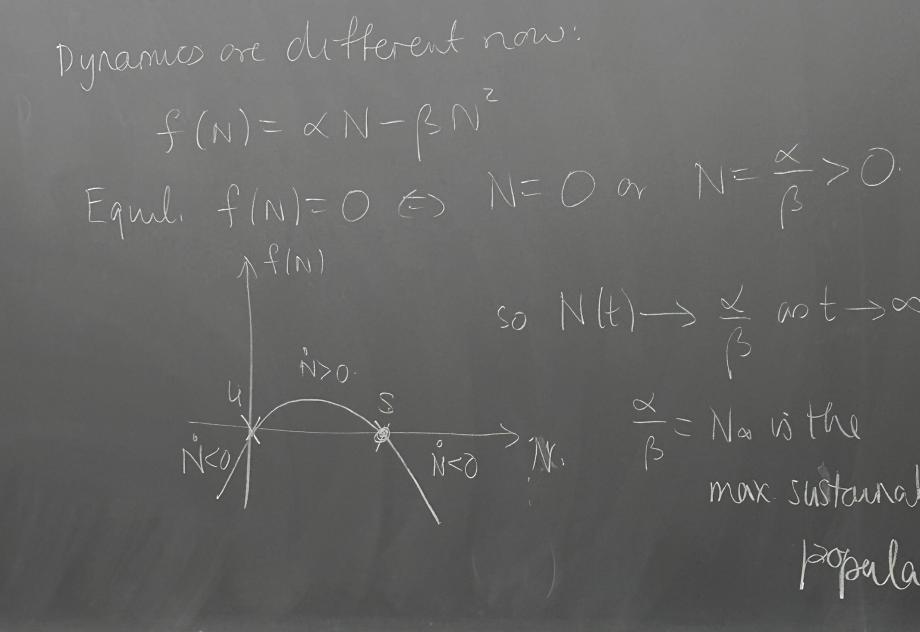
\includegraphics[width=0.6\textwidth]{Figures/lecture1/lec1-4.png}\]
Hence we expect $N(t)$ to tend towards the equilibrium at $\alpha/\beta$. We call $N_\infty = \frac{\alpha}{\beta}$ as the maximum sustainable population.\\

Let's also look at \textbf{spatial effects}, suppose we have an island $\Omega$ where the population is on the island:
\[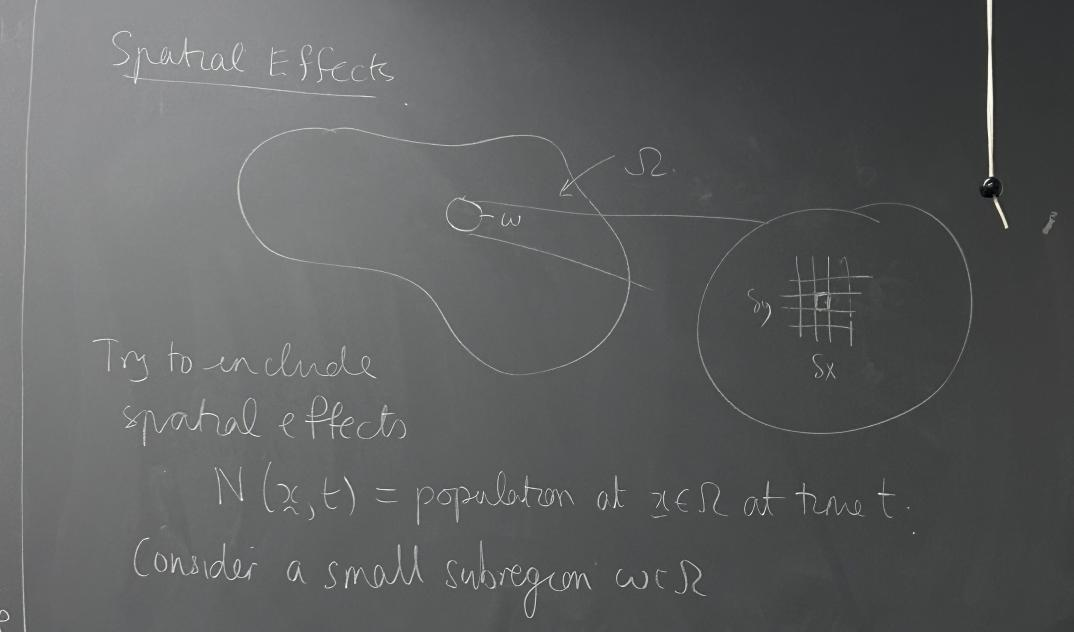
\includegraphics[width=0.6\textwidth]{Figures/lecture1/lec1-5.png}\]
We want $N(x, t)$ to be the population at $x \in \Omega$ and time $t$. Consider a small subregion $\omega \subset \Omega$, and let's let $N_w(t)$ be the population in $\omega$ at time $t$, note that
\[N_w(t) = \int_{w} N(x, t) dx\]
By the principle of conservation of people, we need to take account of the birth and death rate and the immigration rate on the boundary:
\[N_w(t + \delta t) = N_w(t) + \delta t \int_w dx \left(\alpha N(x, t) - \beta N(x, t)^2 \right) - \{\text{immigration at $\partial \omega$ during $(t, t + \delta t)$}\} \]
Let's call a small arc of the boundary as $\delta s$, we make the assumption that people go from more dense place to less dense places.\\

Let's define a flux $\sigma(x, t)$ which is proportional to the spatial gradient $-\nabla N(x, t)$ (the minus sign is here since we are going from more dense places to less dense places). So we write our \textbf{constructive equation}
\[\sigma(x, t) = - \gamma \nabla N, \gamma > 0\]

Hence, the outflow across $\delta s << 1$ should be $\delta s \sigma(x, t) \cdot n$, where $n$ is the unit outward normal vector.
\[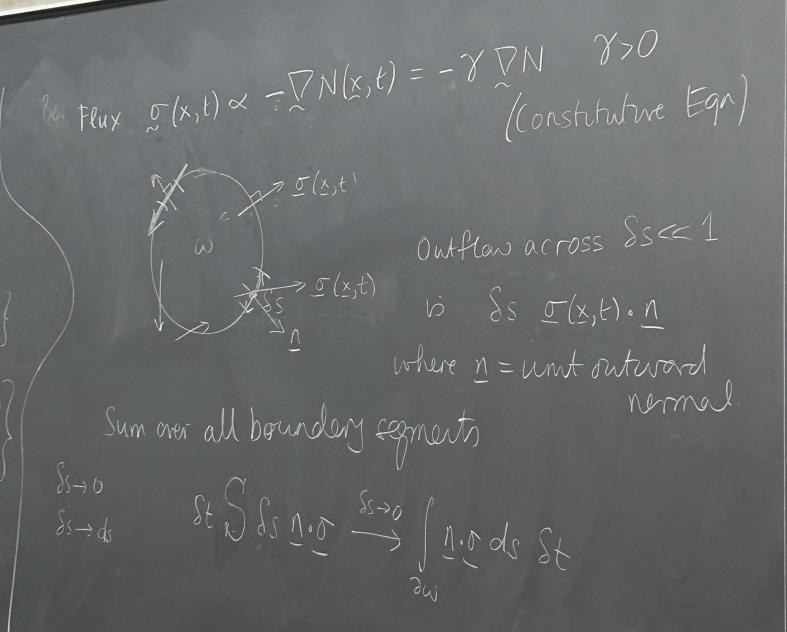
\includegraphics[width=0.6\textwidth]{Figures/lecture1/lec1-6.png}\]
When we sum over all the boundary segments, the immigration effect is 
\[\lim_{\delta s \to 0} \delta t \sum \delta s n \cdot \sigma = \delta t \int_{\partial w} n \cdot \sigma ds \]
Hence, we have that
\begin{align*}
    \int_\omega N(x, t + \delta t) dx &= \int_w N(x, t) dx + \delta t \int_w (\alpha N - \beta N^2) dx - \delta t \int_{\partial w} n \cdot \sigma ds\\
    \iff \int_w \frac{N(x, t + \delta t) - N(x, t)}{\delta t} dx &= \int_w (\alpha N - \beta N^2) dx - \int_w dw \sigma dx \tag*{Divergence Theorem}
\end{align*}
If we take the limit as $\delta t \to 0$ and substitute for $\sigma$, we have that
\[\int_w \frac{\partial N}{\partial t} dx = \int_w (\alpha N - \beta N^2 + \gamma \Delta N) dx\]
for all subregion $w \subset \Omega$. Let ``$w \to 0$" (let the region go smaller and smaller), that is we will divide both side by area of $w$ - $|w|$, and we take $|w| \to 0$:
\[\frac{1}{|w|} \int_w \frac{\partial N}{\partial t} dx = \frac{1}{|w|}  \int_w (\alpha N - \beta N^2 + \gamma \Delta N) dx\]
Assuming $N$ is smooth, taking the limit $|w| \to 0$, we will concentrate at a specific point $x \in w$, gives us
\[\frac{\partial N}{\partial t} = \alpha N - \beta N^2 + \delta \Delta N \text{ in $\Omega$ for $t > 0$}\]
This is called \textbf{Fisher's Equation}. Now we need to supplement this with an initial condition
\[IC: N(x, 0) = N_0(x), x \in \Omega\]
In other words, we should know how many people is at each stop at the beginning. We also need some boundary conditions. The flux at the boundary should be going inward since no one wants to leave the boundary. We want to specify the normal component of the flux should be equal to $0$ on the boundary, hence
\[BC: n \cdot \sigma(x, t) = 0, x \in \partial \Omega\]
Recall that $\frac{\partial N}{\partial n} = n \cdot \nabla N$, hence we have the equivalent condition that
\[\frac{\partial N}{\partial n}(x, t) = 0, x \in \partial \Omega\]
This is an example of a \textbf{reaction-diffusion equation}.
\end{example}

There are no lectures next Wednesday.


\end{document}